\section{Evaluation}

This section presents an in-depth empirical analysis of the design discussed in
Section~\ref{design-section}. To this end, we assess the scalability and
efficiency of the solution using multiple criteria.
%
First, an evaluation of the \textit{strong scaling} behavior of the distributed
algorithm is presented.
%
Second, the \textit{weak scaling} of the solution is assessed with respect to increasing
numbers of targeted latent communities.
%
Next, the effects of \textit{pipelining the computation} and varying the number of latent communities on the system's
performance is analyzed.
%
Further, we evaluate the efficiency and overhead associated with \textit{network
communication} between cluster nodes.
%
Finally, we \textit{contrast} the effectiveness of scaling the computation horizontally
and vertically.

\begin{table*}
  \centering
  \begin{tabular}{l r r l}
    Name            & \#Vertices &       \#Edges & Description \\
    \hline
    com-LiveJournal &  3,997,962 &    34,681,189 & Online blogging social network \\
    com-Friendster  & 65,608,366 & 1,806,067,135 & Online gaming social network \\
    com-Orkut       &  3,072,441 &   117,185,083 & Online social network \\
    com-Youtube     &  1,134,890 &     2,987,624 & Video-sharing social network \\
    com-DBLP        &    317,080 &     1,049,866 & Computer science bibliography collaboration network \\
    com-Amazon      &    334,863 &       925,872 & Product co-purchasing network \\
    \hline
  \end{tabular}
  \caption{Summary of SNAP graph data sets used for evaluation.}
  \label{tab-datasets}
\end{table*}

Empirical results were obtained by performing experiments on the VU and TU/D
DAS5 clusters which consist of 68 and 48 compute nodes respectively. Each
compute node is equipped with a dual 8-core Intel Xeon E5-2630v3 CPU clocked
at 2.40GHz, 64GB of memory and 8TB of storage. Moreover, the compute nodes of
each site are interconnected by
FDR~InfiniBand. All of the experiments reported in this section utilized
publicly available graphs from the Stanford Large Network Dataset
Collection~(SNAP) \cite{snapnets}. Table~\ref{tab-datasets} lists the
collection of data sets used.

%################################################
\subsection{Strong scaling}

\begin{figure*}[t] % [htb]
  \centering
  \epsfig{file=plots/sweep-over-np-fixed-K.eps, width=\textwidth}
  \caption{(a) Execution time of 2048 algorithm iterations for the
  same problem size (com-Friendster, K=1024, M=16384 n=32) across different
  cluster sizes. (b) Speedup achieved for same experiments in (a) with respect to
  8-nodes}
  \label{fig-strong-scaling}
\end{figure*}

In order to evaluate the horizontal scalability of the distributed
implementation we tested the system's performance across different cluster
sizes while holding the problem size constant. For this study, we used the
com-Friendster graph as it contains the largest number of vertices and edges.
%
Figure~\ref{fig-strong-scaling}-a presents the execution time of 2048 algorithm
iterations across multiple cluster sizes. The x-axis starts from 8 worker nodes
as the data set is too large to fit into the collective memory of a smaller
cluster.
%
As shown in the figure, the execution
time steadily decreases by increasing the cluster size.
A deeper analysis of the individual execution phases of the algorithm provides
insights into the scalability if its building blocks.
%
In addition to the total execution time, Figure~\ref{fig-strong-scaling}-a
presents the cumulative time spent in individual computational phases across
iterations. Moreover, Figure~\ref{fig-strong-scaling}-b presents the speedup
achieved for the same experiments reported in
Figure~\ref{fig-strong-scaling}-a. As is clearly shown, the dominant phase of
the execution is update\_pi.
The reported total time for each cluster size is significantly less than the
sum of the execution times of the individual phases. This is due to the
overlapping execution of the two most expensive phases, namely, update\_pi and
deploy\_minibatch. Both of these phases initially gain significant speedup with the
addition of compute nodes. However, the speedup curve gradually slows down for
larger cluster sizes as the work granularity of each worker node decreases,
limiting their resource utilization.
%
The time spent in update\_beta remains relatively constant across cluster sizes
as it performs an insignificant amount of work compared to the synchronization
overhead of a collective MPI reduction operation contained within it.

%################################################
\subsection{Weak Scaling}

\begin{figure*}[t] % [htb]
  \centering
  
\epsfig{file=plots/sweep-over-K-proportional-np.eps, width=\textwidth}
  \caption{(a) Average execution time per algorithm iteration varying
  the number of latent communities proportionally to the number of compute
  nodes. (b) The exact number of communities used for each data point in (a).}
  \label{fig-weak-scaling}
\end{figure*}

A study of a system's weak scaling aids in the assessment of the communication
and synchronization overheads associated with the management of large clusters.
Similarly, it can expose complex issues that hinder performance at scale such
as load imbalance. To fairly evaluate the algorithm's weak scaling behavior we
conducted several executions varying the cluster size and the number of latent
communities proportionally. This methodology ensures that each compute node
performs a relatively constant amount of computational work across all
configurations. However, the number and size of messages exchanged between the
nodes would vary significantly. Figure~\ref{fig-weak-scaling}-a presents the
average execution
time per algorithm iteration across different cluster sizes. On the other hand,
Figure~\ref{fig-weak-scaling}-b reports the set number of communities for each
cluster configuration. The relative change in the average execution time per
iteration is insignificant even though the communication intensity increases
for larger cluster sizes. This observation verifies that the system's overall
overhead is minimal. Additionally, the experimental results shows that the
implementation is capable of achieving good speedups provided the input problem
is large enough for the given cluster size.

%################################################
\subsection{Pipeline efficiency}

\begin{figure}[t] % [htb]
  \centering
  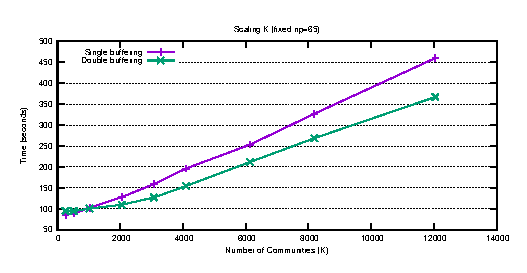
\epsfig{file=plots/sweep-over-K-fixed-np.eps, width=\columnwidth}
  \caption{Performance effect of varying the number of communities on the
    algorithm's execution time on 64-nodes when using single- or
    double-buffering.}
  \label{fig-pipeline}
\end{figure}

As discussed in Section~\ref{design-section}, the collective memory of all
worker nodes serves as the storage for the state of the computation. As such,
the rows of $\pi$ are equally and statically partitioned across all workers.
Given that $\pi$ accesses are random, a node in a cluster of size $C$ must
fetch $(C-1)/C$ of all read requests over the network. Therefore, large cluster
configurations exhibit higher bandwidth demands and are more sensitive
to network latency. To reduce the negative effects of network latency on the
computation, a pipelining scheme was devised to prefetch data dependencies.
Figure~\ref{fig-pipeline} presents the execution time of 1024 algorithm
iterations on a 64-node cluster with double-bufferring enabled and disabled.
Naturally, increasing the number of communities causes a proportional increase
in execution time. However, when double-buffering is enabled, some of the
incurred network latency is hidden by overlapping it with computation.
Moreover, since both computation time and network latency increase with larger
$K$, the benefit of pipelining increases. This can be observed through the
widening gap between both lines depicted in Figure~\ref{fig-pipeline}.

%################################################
\subsection{Horizontal vs. Vertical Scalability}
\begin{figure}[t] % [htb]
  \centering
  
\epsfig{file=plots/hpc-cloud.eps, width=\columnwidth}
  \caption{Performance comparison between the distributed implementation
  running on DAS5 and the multi-threaded solution on machine with 40-cores and
  1TB of RAM.}
  \label{fig-scale-up}
\end{figure}
One of the main drawbacks of designing a distributed solution for a given
algorithm is the inherent complexity of communication and synchronization. A
slightly simpler approach would be developing a multi-threaded version and
running it on a machine with abundant memory and CPU cores. In such a context,
access to all of the algorithm's state would be an order of magnitude faster
than RDMA. Additionally, the overhead associated with synchronizing threads is
negligible compared to using MPI primitives. To evaluate the efficacy of both
approaches we utilized SURFsara's HPC Cloud system to instantiate a virtual
machine with 40~CPU cores and 1TB of memory. The physical machine underlying
the HPC Cloud system contains 40-CPU cores and does not oversubscribe
resources. Therefore, by provisioning all 40~cores we ensured that there is no
resource contention from other users of the system. Figure~\ref{fig-scale-up}
reports the execution time per algorithm iteration for two experimental setups.
Namely, using the HPC Cloud system compared to using 64-nodes of the DAS5
cluster. Clearly, the parallel and distributed implementation vastly
outperforms the single-node multi-threaded solution. Moreover, the trajectory
of both curves shows a widening gap between them suggesting that the relative
performance difference will increase for larger $K$.
%
In conclusion, the overhead of network communication in the distributed version
is more than compensated by the increasing compute power compared to a
a single-node implementation.

%################################################
\subsection{Cluster Communication Efficiency}

%################################################
\subsection{Convergence of Large Datasets}
\begin{figure*}[t] % [htb]
  \centering
  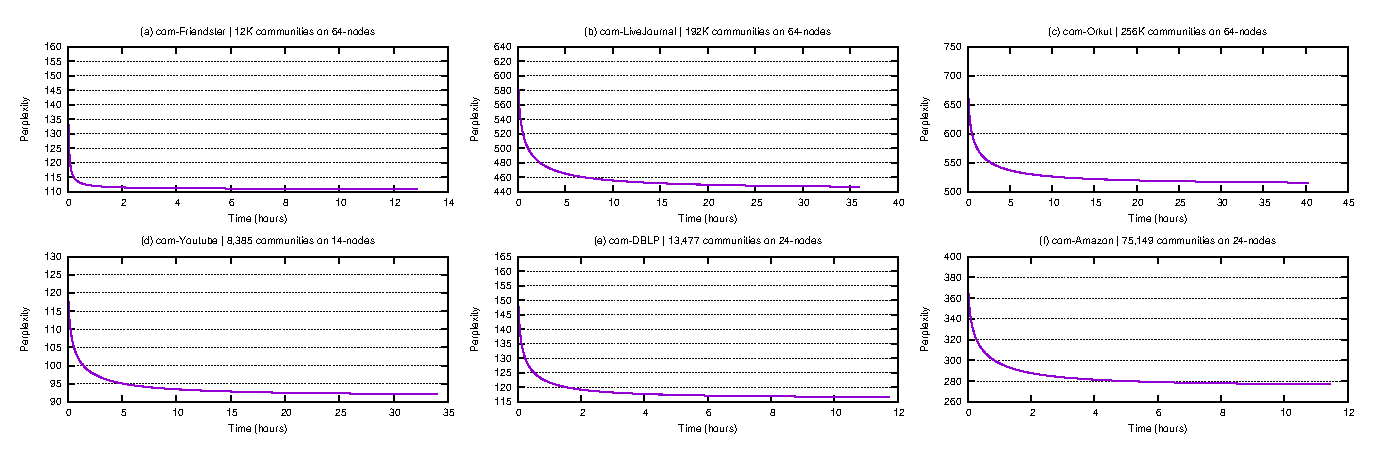
\epsfig{file=plots/ppx.eps, width=\textwidth}
  \caption{FIXME}
  \label{fig-ppx}
\end{figure*}

